The study of the Higgs sector continues to be a major part of the HEP physics program, and will continue to be for 
the next 10 - 20 years.
The full exploration of this sector will require the combination of the upgraded, high luminosity LHC plus precision
results from a lepton collider. The lepton collider that is closest to being realized is the International Linear Collider
in Japan. UTA has been engaged, since 2002, in studies for the SiD Detector Concept for the ILC. 
This work has been an investment in the future of HEP for our group, and is 
consistent with our approach of having an involvement in each generation of colliders. The SiD Detector Concept
was one of two designs validated by the International Detector Advisory Group.
Since 2012, White has served as co-Spokesperson for SiD, with co-Spokesperson Marcel Stanitzki(DESY).
The SiD design study achieved an important milestone with the production of the Detailed Baseline 
Design (DBD) ~\cite{SiDDBD} together with the TDR for the ILC Accelerator. 
The DBD is a compreshensive statement of an advanced detector design ( see Figure~\ref{fig:SiD_Detector} (left)) ~\cite{SiDDet} that will
enable the study of a full range of TeV scale physics. This includes precision Higgs 
measurements, a detailed study of top physics, which is closely connected to the
phenomenon of electroweak symmetry breaking, and a sensitive probe of new physics, such as that from 
additional gauge bosons and extra dimensions at high mass scales, in a program that is complimentary
to that at the LHC. The reach of the ILC in precision measurements of Higgs couplings is shown in 
Figure~\ref{fig:SiD_Detector} (right). The branching ratio for Higgs to invisible decays can be probed at the 1/2\% level 
at the ILC. This is the level at which theoretical studies (Ref. xx) show that significant effects from new physics can be expected.
The ILC is thus a discovery machine both through direct searches and precision measurements.

\begin{figure}[htb]
\centering

      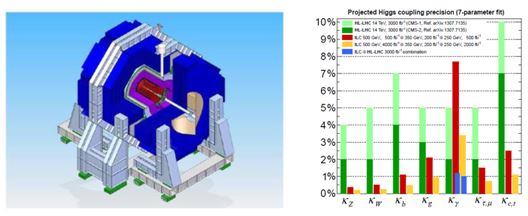
\includegraphics[scale=0.8]{Figures/SiD_Detector_ILC_Higgs.jpg}
      \label{fig:SiD_Detector}

\caption{(left) The SiD Detector (right) Higgs couplings projection for ILC and LHC.}
\end{figure}

Since the writing of the DBD, many further physics and detector optimization studies have been carried
out, including the following areas:
\begin{itemize} [noitemsep,nolistsep]
\item {\bf Pixel tracker option.} Studies of the benefits of a coherent pixel technology implimentation for the
vertex detector and silicon tracker combination.
\item {\bf Hadron calorimeter} New baseline technology choice for the hadron calorimeter: scintillator/steel instead of RPC/steel.
UTA's role in the SiD hadron calorimeter is discussed in the next section.
\item {\bf Flux return/muon steel} Redesign of the solenoid flux return to reduce the external field and facilitate easier handling
and transportation of steel components. 
\item {\bf Backgrounds} Studies of the effects of pair, $ \gamma\gamma $, and beam muon backgrounds on reconstruction of tracks, jets.
\item {\bf Multiplicity studies} Evaluation of the required pipeline depth for the KPix chip - used in all systems except the vertex
 detector.
 \item {\bf Foward region} Redesign of the LumiCal, BeamCal, and other components to reflect the new common L* for SiD and ILD.
 \item{\bf SiD Simulation} A complete reworking of the SiD simulation in the DD4HEP framework - with UTA providing the details
 of the hadron calorimeter.
 \end{itemize}
 
Recently, SiD decided to form the SiD Consortium to formalize the membership of this pre-collaboration.
SiD now has 30 institutions from the U.S.(55\%), Europe (40\%) and Asia (5\%).
We have a set of rules for membership, application procedures for potential new members, and an Institutional
Board that meets at each major ILC event. As SiD Spokesperson White has the following roles:

\begin{itemize} [noitemsep,nolistsep]
\item {\bf Overall Leadership.} Responsible for the physics and technical leadership of the SiD Detector 
Concept, including appointment of sub-group leaders and promotion of SiD within the Linear Collider 
and High Energy Physics community within the U.S. and worldwide.
\item {\bf Head of the SiD Executive Committee.} Responsible for the overall strategy and guidance of 
the SiD Consortium, and calling and chairing weekly meetings.
\item {\bf SiD Representation} External committees and at ILC conferences. SiD Spokespersons are members of, 
or report to, a number of external committees such as the Executive Committee of the Physics and Detectors section of the 
Linear Collider Organization.
\item{\bf Americas Linear Collider Committee} White also serves as the at-large universities' representative on the 
Americas Linear Collider Committee.
\end{itemize}

In their report, P5 described the ILC physics case as "extremely strong", and support for the ILC Project was included
in all scenarios. Earlier a HEPAP Facilities Panel (on which White served) concluded that "The ILC accelerator and detectors 
enable a research program that will address questions of very great scientific importance, and both the accelerator and the detectors 
are {\it absolutely central.}". The Project is currently under evaluation by the Japanese MEXT organization. Recently a 
U.S. DoE - MEXT Working Group was established, and a list of priority areas identified for focus while the project is under evaluation.
There is very strong political, industrial, and community support for the ILC in Japan and a decision is expected in the next
2 years. There has been a series of high-level political and industrial visits by Japanese delegations to the U.S. and White 
has participated as a representative of the U.S. HEP community. ICFA has restructured the Linear Collider Collaboration with
a format designed to carry the project through the next period prior to the final construction decision. If the ILC project is
to be realized, the involvement of the U.S. is essential - there simply is not the required cryomodule production capacity in the rest
of the world. In order to prepare for potential participation, it is therefore critical that the U.S. maintain its long term intellectual
leadership in the project by continued investment in Physics and Detector studies.


